%%
%% This is file `sample-manuscript.tex',
%% generated with the docstrip utility.
%%
%% The original source files were:
%%
%% samples.dtx  (with options: `manuscript')
%% 
%% IMPORTANT NOTICE:
%% 
%% For the copyright see the source file.
%% 
%% Any modified versions of this file must be renamed
%% with new filenames distinct from sample-manuscript.tex.
%% 
%% For distribution of the original source see the terms
%% for copying and modification in the file samples.dtx.
%% 
%% This generated file may be distributed as long as the
%% original source files, as listed above, are part of the
%% same distribution. (The sources need not necessarily be
%% in the same archive or directory.)
%%
%% The first command in your LaTeX source must be the \documentclass command.
%%%% Small single column format, used for CIE, CSUR, DTRAP, JACM, JDIQ, JEA, JERIC, JETC, PACMCGIT, TAAS, TACCESS, TACO, TALG, TALLIP (formerly TALIP), TCPS, TDSCI, TEAC, TECS, TELO, THRI, TIIS, TIOT, TISSEC, TIST, TKDD, TMIS, TOCE, TOCHI, TOCL, TOCS, TOCT, TODAES, TODS, TOIS, TOIT, TOMACS, TOMM (formerly TOMCCAP), TOMPECS, TOMS, TOPC, TOPLAS, TOPS, TOS, TOSEM, TOSN, TQC, TRETS, TSAS, TSC, TSLP, TWEB.
% \documentclass[acmsmall]{acmart}
\documentclass[sigchi,authordraft]{acmart}

%% 追加
\usepackage{bm}
\newcommand\figref[1]{\textbf{Figure~\ref{fig:#1}}}
\newcommand\tabref[1]{\textbf{Table~\ref{tab:#1}}}
\usepackage{url}
\usepackage{color}
\usepackage{multirow}
%% ここまで

%%%% Large single column format, used for IMWUT, JOCCH, PACMPL, POMACS, TAP, PACMHCI
% \documentclass[acmlarge,screen]{acmart}

%%%% Large double column format, used for TOG
% \documentclass[acmtog, authorversion]{acmart}

%%%% Generic manuscript mode, required for submission
%%%% and peer review
% \documentclass[manuscript,screen,review]{acmart}
%% Fonts used in the template cannot be substituted; margin 
%% adjustments are not allowed.
%%
%% \BibTeX command to typeset BibTeX logo in the docs
\AtBeginDocument{%
  \providecommand\BibTeX{{%
    \normalfont B\kern-0.5em{\scshape i\kern-0.25em b}\kern-0.8em\TeX}}}

%% Rights management information.  This information is sent to you
%% when you complete the rights form.  These commands have SAMPLE
%% values in them; it is your responsibility as an author to replace
%% the commands and values with those provided to you when you
%% complete the rights form.
\setcopyright{acmcopyright}
\copyrightyear{2018}
\acmYear{2018}
\acmDOI{10.1145/1122445.1122456}

%% These commands are for a PROCEEDINGS abstract or paper.
\acmConference[Woodstock '18]{Woodstock '18: ACM Symposium on Neural
  Gaze Detection}{June 03--05, 2018}{Woodstock, NY}
\acmBooktitle{Woodstock '18: ACM Symposium on Neural Gaze Detection,
  June 03--05, 2018, Woodstock, NY}
\acmPrice{15.00}
\acmISBN{978-1-4503-XXXX-X/18/06}


%%
%% Submission ID.
%% Use this when submitting an article to a sponsored event. You'll
%% receive a unique submission ID from the organizers
%% of the event, and this ID should be used as the parameter to this command.
%%\acmSubmissionID{123-A56-BU3}

%%
%% The majority of ACM publications use numbered citations and
%% references.  The command \citestyle{authoryear} switches to the
%% "author year" style.
%%
%% If you are preparing content for an event
%% sponsored by ACM SIGGRAPH, you must use the "author year" style of
%% citations and references.
%% Uncommenting
%% the next command will enable that style.
%%\citestyle{acmauthoryear}

%%
%% end of the preamble, start of the body of the document source.
\begin{document}

%%
%% The "title" command has an optional parameter,
%% allowing the author to define a "short title" to be used in page headers.
\title{Pulse Wave Generation Method for PPG by using Display}

%%
%% The "author" command and its associated commands are used to define
%% the authors and their affiliations.
%% Of note is the shared affiliation of the first two authors, and the
%% "authornote" and "authornotemark" commands
%% used to denote shared contribution to the research.

\author{Atsuhiro Fujii}
\affiliation{%
  \institution{Ritsumeikan University}
   \city{Shiga}
   \country{Japan}
}
\email{atsuhiro.fujii@iis.ise.ritsumei.ac.jp}

\author{Kazuya Murao}
\affiliation{%
  \institution{Ritsumeikan University / Japan Science and Technology Agency, PRESTO}
   \city{Shiga}
   \country{Japan}
}
\email{murao@cs.ritsumei.ac.jp}

\author{Naoji Matsuhisa}
\affiliation{%
  \institution{Keio University / Japan Science and Technology Agency, PRESTO}
   \city{Kanagawa}
   \country{Japan}
}
\email{naoji@keio.jp}

%%
%% By default, the full list of authors will be used in the page
%% headers. Often, this list is too long, and will overlap
%% other information printed in the page headers. This command allows
%% the author to define a more concise list
%% of authors' names for this purpose.
\renewcommand{\shortauthors}{Fujii and Murao}

%%
%% The abstract is a short summary of the work to be presented in the
%% article.
\begin{abstract}
  The extensive research on wearable devices has led to devices of various shapes and wearing areas. Wearable devices are often used to record the user's biometric information, and methods to detect physical abnormalities from the acquired data have been proposed. Among biometric data, pulse data has been used in methods such as heart rate monitoring and emotion estimation. The most common type of pulse sensor is the photoplethysmogram (PPG), which irradiates a green LED on the skin and measures pulse data from changes in the light reflected through the blood vessels. PPG sensors have been implemented in commercially available wearable devices such as smartwatches. The PPG sensor requires blood flow for data acquisition due to the characteristics of the mechanism. When a smartwatch is worn on an artificial body such as a prosthetic hand or a robotic arm, correct data cannot be acquired because there is no blood flow. In this study, we propose a method that enables the PPG sensor to measure arbitrary pulse data using a display. If this method is successful, it will be possible to input pulse data measured at the junction of the live body and the prosthetic hand to the display, and have the smartwatch attached to the prosthetic hand read the same pulse data. In this paper, we focus on the heart rate and report the results of an experiment in which a target heart rate was input and the display was controlled to determine whether the target heart rate could be obtained by a smartwatch. We implemented a display drawing program and conducted the evaluation using five kinds of smartwatches and four kinds of displays. Results showed that the error between the target heart rate and the heart rate acquired by the smartwatch was within $3$ beats per minute in many cases when the target heart rate was set to 60--100. When the target heart rate was set to 40--55 and 105--200, the heart rate could be input to the smartwatch with a small error under some conditions. We compared the pulse wave status evaluation indices calculated from the real pulse wave obtained from the body and the generated pulse wave, and clarified that the pulse wave could be generated by the proposed method. By comparing the waveforms, the danger of calculating only the indices without checking the waveforms was clarified.
\end{abstract}

%%
%% The code below is generated by the tool at http://dl.acm.org/ccs.cfm.
%% Please copy and paste the code instead of the example below.
%%
\begin{CCSXML}
<ccs2012>
 <concept>
  <concept_id>10010520.10010553.10010562</concept_id>
  <concept_desc>Computer systems organization~Embedded systems</concept_desc>
  <concept_significance>500</concept_significance>
 </concept>
 <concept>
  <concept_id>10010520.10010575.10010755</concept_id>
  <concept_desc>Computer systems organization~Redundancy</concept_desc>
  <concept_significance>300</concept_significance>
 </concept>
 <concept>
  <concept_id>10010520.10010553.10010554</concept_id>
  <concept_desc>Computer systems organization~Robotics</concept_desc>
  <concept_significance>100</concept_significance>
 </concept>
 <concept>
  <concept_id>10003033.10003083.10003095</concept_id>
  <concept_desc>Networks~Network reliability</concept_desc>
  <concept_significance>100</concept_significance>
 </concept>
</ccs2012>
\end{CCSXML}

\ccsdesc[500]{Computer systems organization~Embedded systems}
\ccsdesc[300]{Computer systems organization~Redundancy}
\ccsdesc{Computer systems organization~Robotics}
\ccsdesc[100]{Networks~Network reliability}

%%
%% Keywords. The author(s) should pick words that accurately describe
%% the work being presented. Separate the keywords with commas.
\keywords{datasets, neural networks, gaze detection, text tagging}

%% A "teaser" image appears between the author and affiliation
%% information and the body of the document, and typically spans the
%% page.
% \begin{teaserfigure}
%   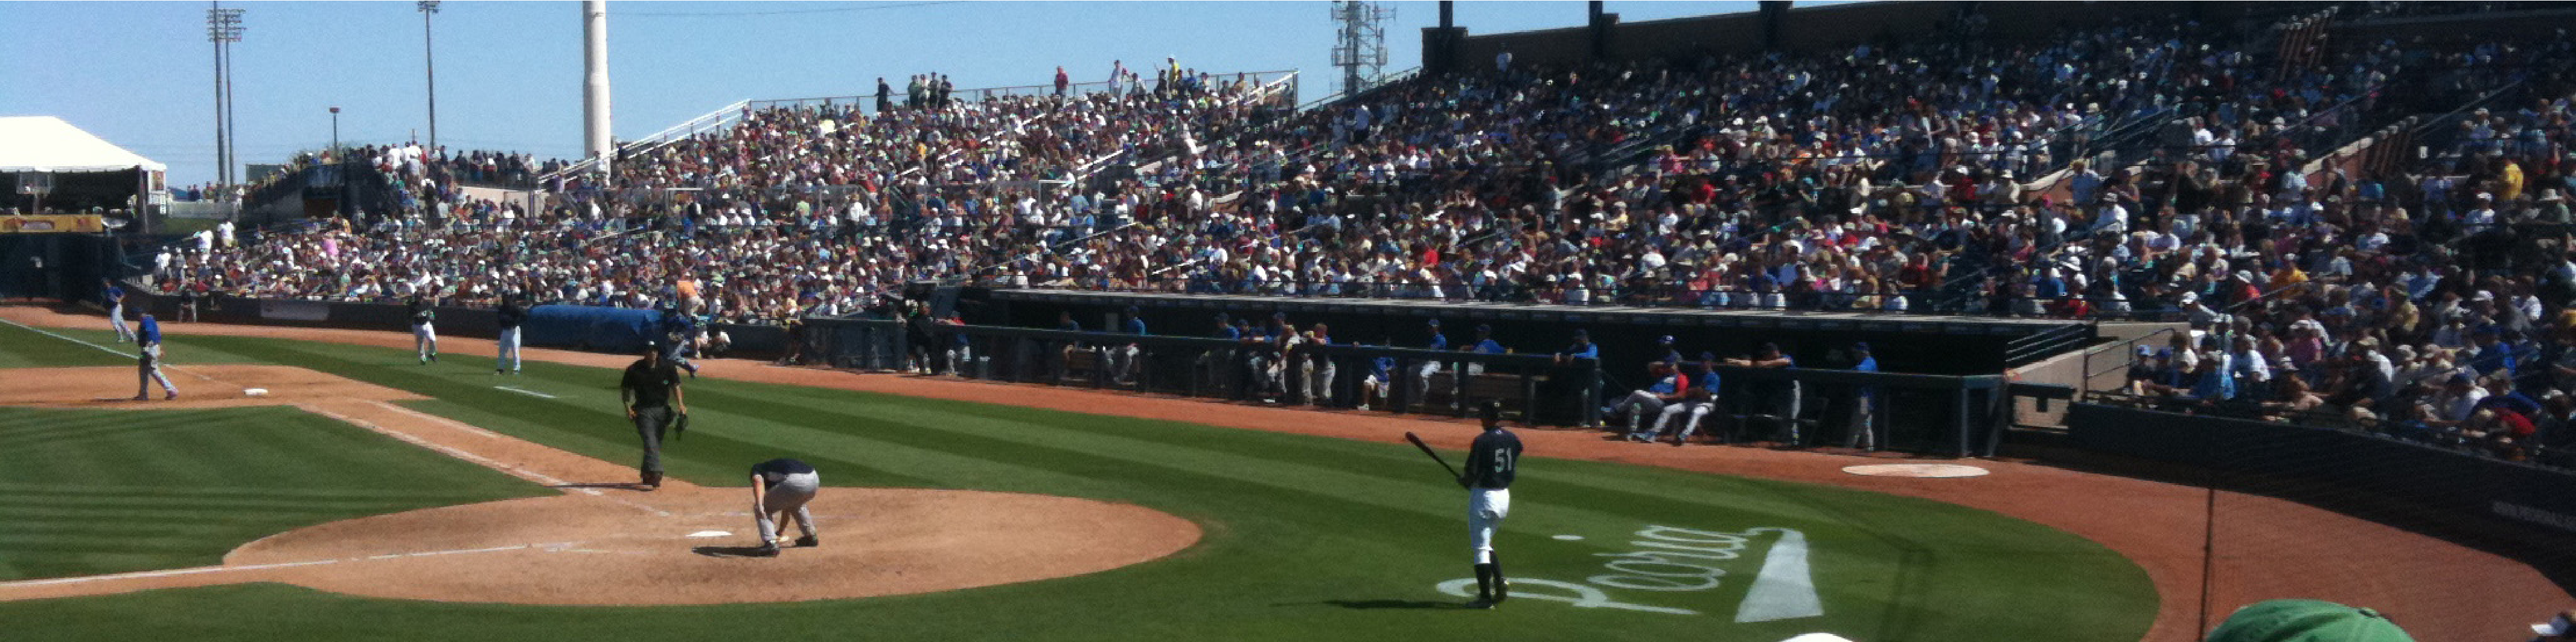
\includegraphics[width=\textwidth]{sampleteaser}
%   \caption{Seattle Mariners at Spring Training, 2010.}
%   \Description{Enjoying the baseball game from the third-base
%   seats. Ichiro Suzuki preparing to bat.}
%   \label{fig:teaser}
% \end{teaserfigure}

%%
%% This command processes the author and affiliation and title
%% information and builds the first part of the formatted document.
\maketitle

% 1
\section{Introduction}
\label{sec:introduction}
With the growing awareness of health management, wearable devices that record biometric information have become widely used. The biometric information to be recorded includes a variety of data such as activity, respiratory rate, body temperature, cardiac potential, blood pressure, gaze, pulse wave, and heart rate. The pulse sensor used to acquire these latter two (pulse wave and heart rate) irradiates the skin with LEDs that emit infrared light, red light, or light with a green wavelength around 550 nm. The oxidized hemoglobin in the blood flowing through arteries can absorb these lights. The pulse sensor takes advantage of the fact that the amount of reflected light decreases as the arterial blood flow increases with the timing of the heartbeat, and uses a phototransistor to acquire changes in the amount of reflected light and measure the pulse wave. The pulse wave data is numerical data of the change of the reflected light, and the heart rate is measured by detecting the peak appearing in the pulse wave data. This type of pulse wave measurement technique is called photoplethysmography (PPG). Many commercially available wearable devices (e.g., smartwatches) are equipped with a PPG sensor as a pulse sensor.\par

We speculate that it may be possible to measure an arbitrary pulse wave by giving a change of light to the PPG sensor. In this paper, we propose disp2ppg, a method that enables the PPG sensor to acquire pulse data using a display. Paul et al. \cite{ppg_generator} developed a hardware PPG simulator using an LED array to generate PPG signals, which was designed to simplify the data collection for photoplethysmography imaging (PPGI). Our disp2ppg method differs in that it aims to use a small device to input data to a PPG sensor equipped on a wearable device. Specifically, it utilizes a smartwatch to measure an arbitrary heart rate. We set two objectives for disp2ppg: PPG transfer and fake PPG.\par

In terms of PPG transfer, artificial bodies such as prosthetic hands, robotic arms, and telepresence robots do not have any blood flow, which means it is not possible to measure the biometric data even if a smartwatch is worn on the wrist. While smartwatch functions such as calling, messaging, clocking, and payment, as well as sensors such as accelerometers and GPS, can be used in artificial bodies the same as in the living body, pulse data cannot be measured. When a smartwatch is attached to other body parts where blood flow exists (e.g., the ankle) in order to measure pulse data, the usability of other functions (e.g., messaging) is reduced. Other possible methods for PPG transfer include attaching an additional PPG sensor to other body parts where blood flow exists and inputting PPG data wirelessly to the smartwatch, or detecting PPG data (or heart rate data) from sensors other than the PPG \cite{Biowatch, heart_rate_accelerometer, SeismoTracker}. However, since most of the publicly available applications that use PPG data read the values from PPG sensors equipped on the device, PPG data collected by these methods may not be usable for many applications. With the proposed method, even when a smartwatch is attached to an artificial body, it can read the person's pulse data by changing the light of the display under its PPG sensor in accordance with the pulse data measured at the junction of the living body and the prosthetic hand. It is thus possible to use the normal functions of the smartwatch since it is not modified and only the display is mounted on the artificial body. Users can compare various items such as the design, function, and weight of commercial smartwatches and use the model of their choice. In addition, the PPG sensor on the smartwatch acquires the data, without modifying the smartwatch, thus allowing the user to use common applications. When applied to a remote robot avatar, the operator's biometric data can be measured on the avatar's body.\par

As for fake PPG, if the PPG sensor measures an arbitrary heart rate by the proposed method, it might be possible for a malicious user to falsify the heart rate and pretend to be exercising or continuing to rest. If a device that utilizes the proposed method becomes widely feasible and has a significant social impact, it will be necessary to discuss the use of the current PPG sensor from the viewpoint of its vulnerability.\par

In the following sections, we introduce related works in Section \ref{sec:related} and explain the details of the proposed method in Section \ref{sec:method}. Section \ref{sec:evaluation} discusses the evaluation of the proposed method, Section \ref{sec:limitation} describes limitations of the proposed method, and finally Section \ref{sec:conclusion} concludes the paper.



% 2
\section{Related Work}
\label{sec:related}
In this section, we introduce research on sensing with wearable devices, the use of smart watches, and the use of pulse data.

% 2.1
\subsection{Sensing with wearable devices}
Ham et al.\cite{smart_wristband} have proposed a wristband-type device as an input device for smart glasses. This device is equipped with a touch panel and an inertial measurement unit, and can be operated by touch or a motion such as a twist of the wrist. Since the device can be used by wearing it on the wrist, the user's movement is not restricted and has a high degree of freedom. A touch panel was used for pointing to improve the stability of the input.
Hernandez et al.\cite{bioglass} propose a method for recognizing pulse rate and respiration rate from data obtained from the accelerometer, gyroscope, and camera built into Google Glass, a head-worn wearable device.
Nishajith et al.\cite{smart_cap} designed and implemented Smart Cap as a wearable device to assist the visually impaired with situational awareness. The device consists of a Raspberry Pi 3, a Raspberry Pi NoIR Camera V2, an earphone, and a power supply. The Raspberry Pi NoIR (No Infrared) Camera V2 is an infrared camera module for the Raspberry Pi. The object detected in the image obtained by this infrared camera is described by voice through an earphone.
These are all researches on wearable devices that are worn on body parts, and researches using devices of various shapes have been conducted.\par

There are various body parts where wearable devices are worn.
Vahdatpour et al.\cite{localization_vahdatpour} had 25 subjects wear accelerometers at 10 locations on the forearm, upper arm, head, thigh, shin, and waist, and collected acceleration data during daily activities. From the collected data, the SVM (Support Vector Machine) was used to estimate the attachment site with an average accuracy of 89\%.
Sztyler et al.\cite{localization_sztyler} attached accelerometers to seven locations on the head, chest, left upper arm, left wrist, waist, left pocket of pants, and left ankle of 15 subjects and collected acceleration data during various physical activities. From the collected data, the wearing site was estimated using Random Forest, and an average accuracy of 89\% was achieved.
Kunze et al.\cite{localization_kunze} attached accelerometers to four locations on the wrist, the right side of the head above the eyes, the left trouser’s pocket, and the left breast pocket of six subjects and collected data during walking movements. From the collected data, the attachment site was estimated using the C4.5 classifier.
We have proposed a method to estimate the body part where the wearer is wearing a wearable device without having the wearer perform a specific action, using ECG and pulse data, which are biometric information that can be acquired by the wearable device.\cite{localization_yoshida}\par

As described above, wearable devices have been proposed in various shapes. Because of the wide range of wearing sites, research using wearable devices has been actively conducted.


% 2.2
\subsection{Studies using Smartwatches}
Among wearable devices, smartwatches have been commercially available for a long time, and many researches have been conducted.
Spinsante et al.\cite{accuracy_in_low_intensity} focused on the heart rate obtained from a smartwatch during low-intensity physical activity and measured its accuracy.
Sen et al.\cite{eating_recognition} propose a method to record eating behavior, such as whether the user ate with hands, chopsticks, or a spoon, using data obtained from the accelerometer and gyroscope of a smartwatch. By capturing food images with the camera built into the smartwatch and performing image identification, the contents of the meal are also recorded.
Johnston et al.\cite{smartwatch_walk_authentication} focused on the fact that smartwatches are always worn at the same place and in the same direction, and proposed a method for biometric authentication based on gait using data obtained from the accelerometer and gyroscope of the smartwatch. In general, smartphones are often carried in a trouser pocket or handbag. Compared to these locations, activity information tends to appear more on the wrist where the smartwatch is worn.
Weiss et al.\cite{smartwatch_activity_recognition} showed that a smartwatch can identify actions more effectively than a smartphone in hand-based physical behaviors such as eating. For the behavior ``drinking'', the smartwatch was able to identify the behavior with 93.3\% accuracy, while the smartphone could only achieve 77.3\% accuracy.
Iakovakis et al.\cite{oh_detection} are conducting a study aimed at predicting the Blood Pressure (BP) drop caused by postural changes using a smart watch. Orthostatic hypotension (OH) has been shown to cause dizziness and fainting, and is a risk factor for falls in the young as well as the elderly. Therefore, they propose a mathematical prediction model which can reduce the risk of fall due to OH by sensing heart rate variability.
Mauldin et al.\cite{smartfall} proposed an Android application ``SmartFall'' that detects falls using acceleration data obtained from a commercially available smartwatch. The smartwatch is paired with a smartphone that runs SmartFall. SmartFall communicates with a cloud server to perform the calculations necessary to predict falls in real time, while maintaining data privacy.
Ciabattoni et al.\cite{smartwatch_stress_detection} have proposed a method for detecting mental stress during various cognitive tasks in real time. Galvanic Skin Response (GSR), RR Interval and Body Temperature (BT) acquired by a commercial smartwatch are used to classify stress.\par

On an artificial body, wearable devices can not collect biometric information and thus we may not be able to use these methods. Methods using sensors such as accelerometers and GPS are applicable, but methods using biometric data are not. We try to make these applications available to artificial bodies as well as to living bodies by inputting data to biometric sensors of wearable devices.


% 2.3
\subsection{Studies using Pulse Data}
Havriushenko et al.\cite{respiratory_rate_estimation} have proposed a method for estimating respiratory rate from pulse wave data using neural networks. To measure respiratory rate, thermal sensor placed in nasal channels or elastic chest belt are often used. However, these devices may interfere with sleep. A method of measuring respiratory rate using pulse wave data can be implemented in a wearable device. As a result of the evaluation, the proposed model provides an average respiratory rate estimation error lower than 2.2 breaths per minute.
Han et al.\cite{arrhythmia_detection} proposed a method for detecting premature atrial contraction (PAC) and premature ventricular contraction (PVC) using PPG data acquired from a smartwatch.
Goshvarpour et al.\cite{emotion_recognition_poincare} have proposed a method for classifying emotional responses by means of a simple dynamic signal processing technique and fusion frameworks. The authors recorded the electrocardiogram and finger pulse activity of 35 participants during rest condition and when subjects were listening to music intended to stimulate certain emotions. After using poincare plots, the SVM was used to classify them into four emotions: happiness, sadness, peacefulness, and fear.
Kajiwara et al.\cite{pulse_order_picking} focus on the fact that many logistics companies adopt a manual order picking system, and that emotions and engagement affect work efficiency and human errors, and propose a method for predicting emotions and engagement during work with high exercise intensity based on behavior and pulse waves acquired by wearable devices. Pulse wave, eye movements, and movements are input to deep neural networks to estimate emotion and engagement. The results of verification experiments showed that emotion and engagement during order picking can be predicted from the behavior of the worker with an accuracy of error rate of 0.12 or less.
Lee et al.\cite{fast_emotion_recognition} have conducted research on improving the speed of emotion recognition using PPG signal. A two-dimensional emotion model based on valence and arousal is adopted, and one-dimensional convolutional neural network (1D CNN) is used to recognize emotion from 1.1 second PPG signal. They tested the 1D CNN as a binary classification (high or low valence and arousal) using the dataset for emotion analysis using physiological (DEAP) signals, and achieved recognition accuracy of 75.3\% for valence and 76.2\% for arousal.\par

Pulse data is one of the most important biological information, as it can detect abnormalities in the body and estimate emotions. Most of the pulse sensors in commercially available wearable devices use photoplethysmogram. Therefore, when a wearable device is worn on an artificial body where blood flow does not exist, pulse data cannot be acquired. We focus on pulse data among biometric data, and propose a method to allow a wearable device to measure pulse data similar to that of a living body even on an artificial body.



% 3
\section{Proposed Method}
\label{sec:method}
This section explains the details of the proposed method.

% 3.1
\subsection{Overview}
\label{subsec:overview}
In our proposed method, when a user sets an arbitrary heart rate, the display lights, and a smartwatch worn on the display measures the specified heart rate. The flow of the proposed method is shown in \figref{method}. First, the real (target) heart rate of the user is obtained with a PPG sensor that is separate from the smartwatch. The proposed method changes the brightness of the display connected to a microcomputer in accordance with the target heart rate. Then, the smartwatch worn over the display measures the heart rate that is the same as the target heart rate.

\begin{figure}[!t]
  \centering
  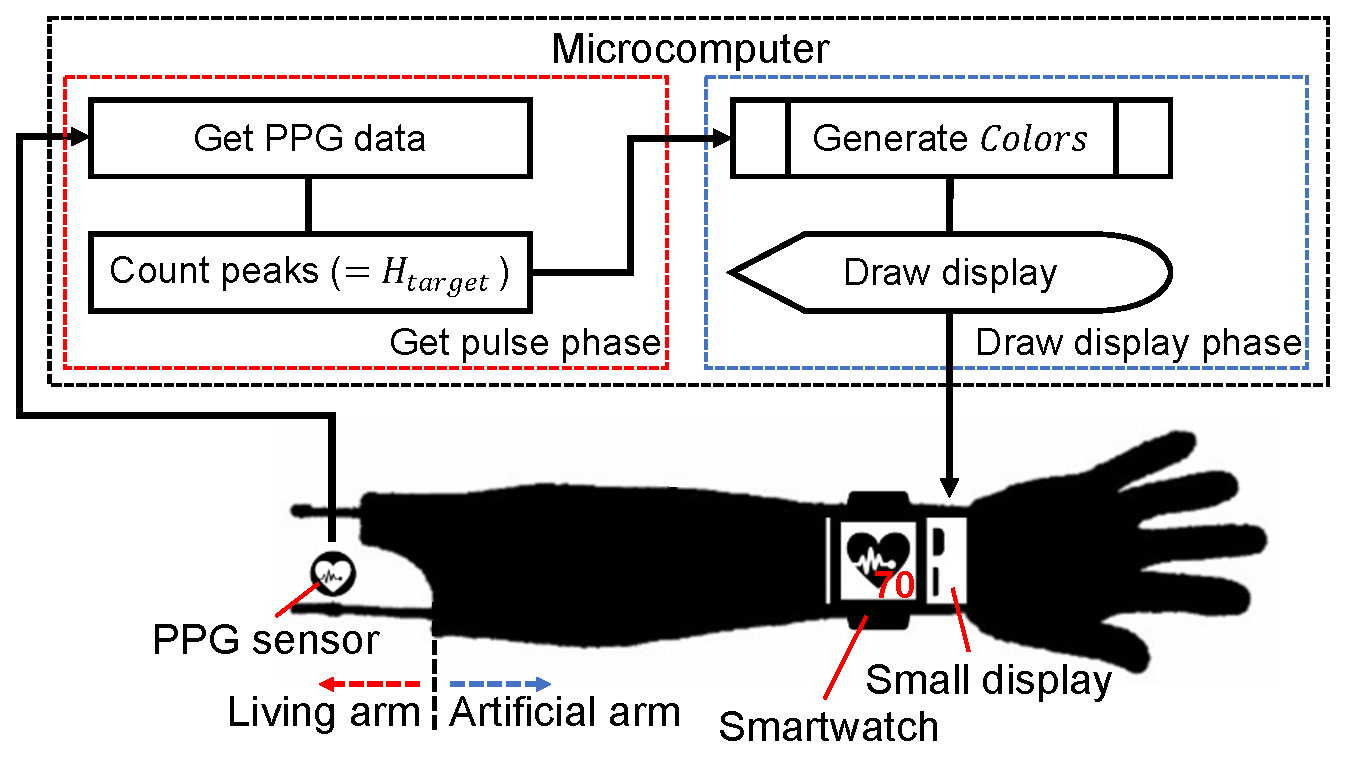
\includegraphics[width=0.75\linewidth]{figures/method.eps}
  \caption{Process flow of proposed method.}
  \label{fig:method}
\end{figure}


% 3.2
\subsection{Target Heart Rate Calculation}
The target heart rate that the proposed method lets the smartwatch measure is the wearer's heart rate obtained using another PPG sensor. Its value can be specified in real time. Let $H_{target}$ be the target heart rate. $H_{target}$ can also be given manually if the user wants the smartwatch to measure a specific heart rate.


% 3.3
\subsection{Display Control}
\label{subsec:display_control}
The brightness of the display is controlled so that the heart rate measured by the smartwatch becomes $H_{target}$. An array $Colors$ that holds the brightness of the display to let the smartwatch detect a single pulse is prepared in advance.\par

The PPG sensors irradiate infrared, red, or green LEDs onto the skin and measure the pulse data from the changes in light reflected through the blood vessels. Because blood flow increases with the timing of the pulse, more light is absorbed by the blood vessels, and the reflected light is dimmer. Since black absorbs more light than white, the more the display is rendered black, the darker the light emitted from the smartwatch worn on the display and reflected through the display.\par

The proposed method draws the values of $Colors$ on the display one by one for each $T$[s]. We set the drawing interval $T$[s] for each value of $Colors$ as follows, so that $Colors$ is played $H_{target}$ times in one minute.
\begin{equation}
  \label{eqn:wait}
  T = 60 / \{len(Colors) * H_{target}\}
\end{equation}
$len(Colors)$ is the data length of $Colors$.


% 3.4
\subsection{Pulse Data Measurement}
In the proposed method, a smartwatch is worn over a blinking display and pulse data is measured. Pulse data measured from a PPG sensor equipped on a smartwatch can be used in various applications. However, the performance of the PPG sensor and the algorithm for measuring the pulse data will vary depending on the model of the smartwatch, and are not disclosed to the public. For this reason, we set the target heart rate manually in our evaluation experiment. We then observe the error between the target heart rate and the heart rate measured by the smartwatch and investigate the effects of the smartwatch model and display.



% 4
\section{Evaluation}
\label{sec:evaluation}
This section describes the experiments we conducted to evaluate the effectiveness of the proposed method. We measured the heart rate acquired by a smartwatch when an arbitrary target heart rate was given.

% 4.1
\subsection{Evaluation Environment}
TicWatch Pro WF12106, PUMA Smartwatch, Apple Watch Series 3 and Series 5, and SMART R F-18 were used for the evaluation experiment. For the display, we used the laptop display of Legion 7 15IMH05 by Lenovo (Display A), two small 3.5-inch displays designed for Raspberry Pi by ELECROW and OSOYOO (Displays B and C), and a lightweight flexible display \cite{flexible_display} (Display D) we made. The smartwatches and displays A, B, and C are shown in \figref{smartwatches}, and Display D is shown in \figref{flexible}.

\begin{figure}[!t]
  \centering
  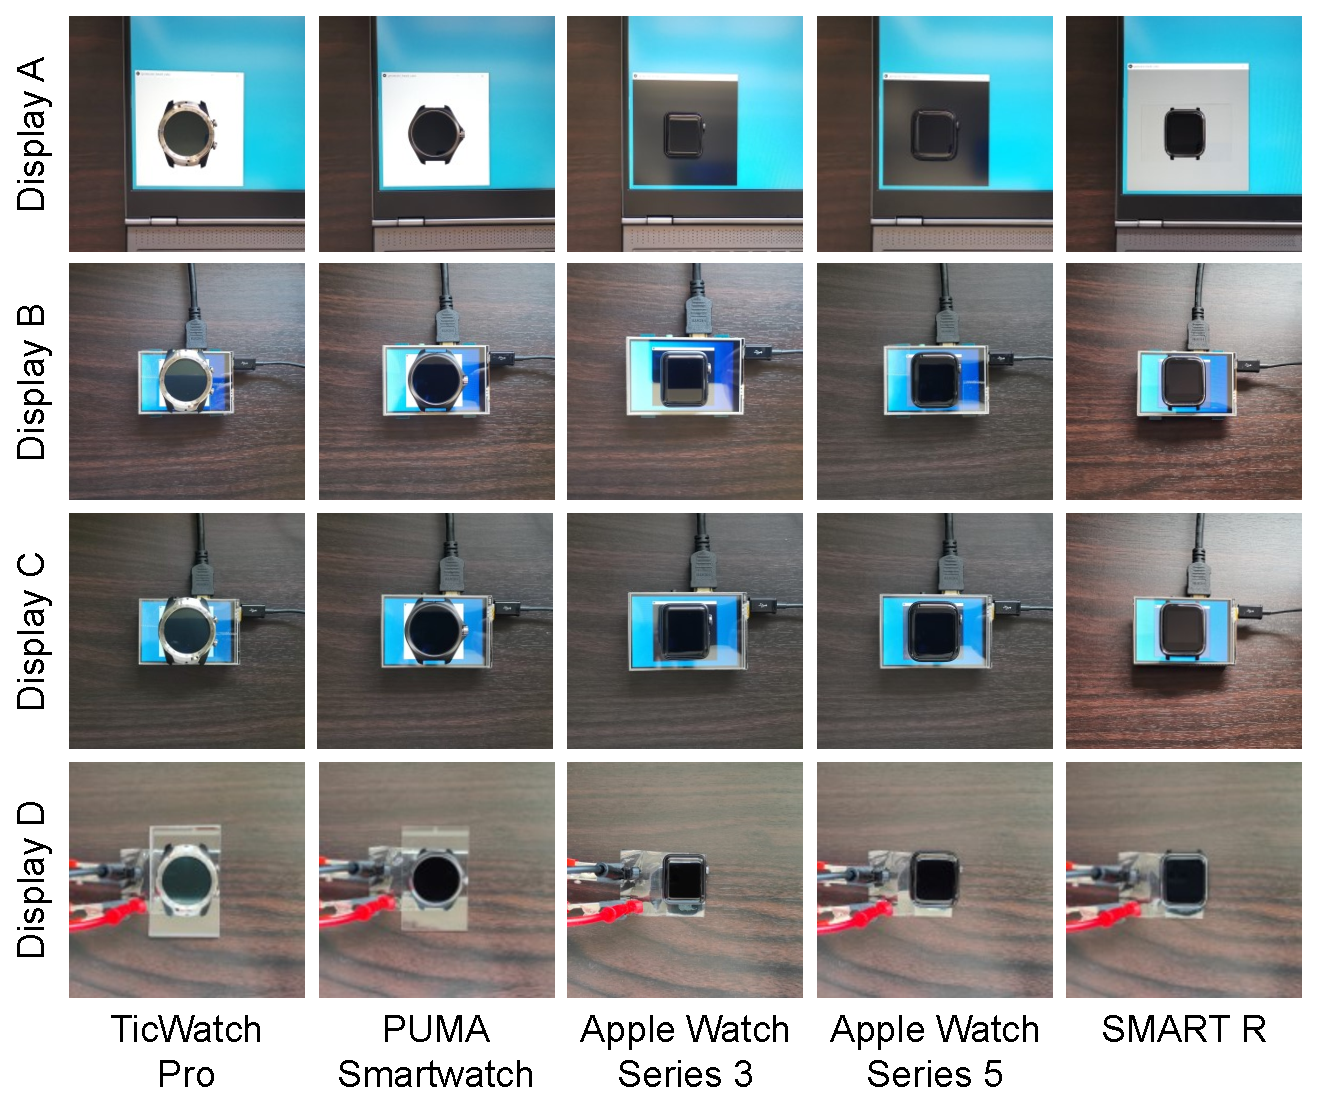
\includegraphics[width=0.78\linewidth]{figures/smartwatches.eps}
  \caption{Smartwatches and displays used in the experiment.}
  \label{fig:smartwatches}
\end{figure}

\begin{figure}[!t]
  \centering
  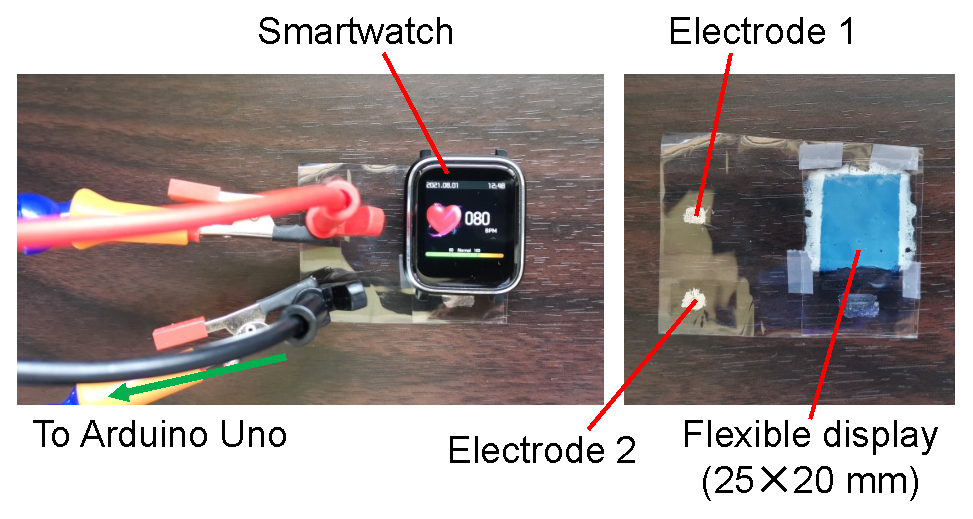
\includegraphics[width=0.75\linewidth]{figures/flexible.eps}
  \caption{Appearance of the flexible display (Display D).}
  \label{fig:flexible}
\end{figure}


% 4.2
\subsection{$Colors$ determination and Display drawing program implementation}
\label{subsec:colors_and_program}
Several displays with different connection methods to the computer were used in the evaluation experiments. In this section, we describe the program we implemented to control them.

% 4.2.1
\subsubsection{Displays A, B, C}
Since Display A is a laptop display and Displays B and C are displays that can be connected using HDMI, these displays are recognized by the computer as regular displays.\par

The $Colors$ data is represented grayscale, a type of computer color representation that uses 256 levels (0--255) to represent shades of color from black to white. $Colors[i]~(i=0,\dots,L)$ whose length is $L$ is generated by the following equation.
\begin{equation}
  Colors[i]=\min\left(\sin\left(\frac{2\pi i}{L}\right)+1,1\right)*SCALE+BASE
\end{equation}
We determined the values of $L$, $SCALE$, and $BASE$ heuristically in advance for each display-smartwatch combination.\par

For example, if $L=19$, $SCALE=30$, and $BASE=225$, then $Colors$ was determined to be the following sequence of numbers.
\begin{equation*}
  \begin{split}
    Colors = [255, 255, 255, 255, 255, 255, 255, 255, 255, 255,\\250, 240, 232, 227, 225, 225, 229, 236, 245, 255]
  \end{split}
\end{equation*}
This $Colors$ is plotted in \figref{colors_wave}. The smaller the grayscale, the closer it is to black.\par

A program to change the brightness and darkness of the display was implemented using Python and Processing. Processing\footnote{\url{https://processing.org}} is a programming language based on Java that excels in visual expression, and is used to create electronic art and visual design. Processing receives the target heart rate from the standard input of Python, it uses \texttt{background} method to draw the grayscale as the background color of the window on the display.

\begin{figure}[!t]
  \centering
  \includegraphics[width=1\linewidth]{figures/colors_wave.eps}
  \caption{Data of light and dark changes in the display that can make a smartwatch detect a single pulse.}
  \label{fig:colors_wave}
\end{figure}

% 4.2.2
\subsubsection{Display D}
Display D is made of a flexible film that can fit on curved areas like the arm or the back of the smartwatch, but it does not have HDMI. It blinks by switching the potential direction applied to the terminals. The color of the display becomes darker when a higher voltage is applied to electrode 1 and lighter when a higher voltage is applied to electrode 2.\par

As a result of the heuristic search in the preliminary study, $Colors$ was determined to be the following sequence of colors.
\begin{equation*}
  \begin{split}
    Colors = [BLACK, WHITE]
  \end{split}
\end{equation*}
For $BLACK$, set the voltage of electrode 1 to 2[V] and the voltage of electrode 2 to 0[V], and for $WHITE$, set the voltage of electrode 1 to 0[V] and the voltage of electrode 2 to 2[V]. \figref{colors_flexible} shows how the voltage changes when the $Colors$ are repeated twice.\par

We implemented a display drawing program using Arduino Uno R3 microcomputer. This microcomputer can control the output voltage by pulse width modulation (PWM). It receives the target heart rate from the standard input of Python running on a computer connected to it and then changes the voltage to the display.

\begin{figure}[!t]
  \centering
  \includegraphics[width=1\linewidth]{figures/voltage_wave.eps}
  \caption{How the voltage changes when the $Colors$ are repeated twice.}
  \label{fig:colors_flexible}
\end{figure}


% 4.3
\subsection{Data acquisition}
\label{subsec:data_acquisition}
A smartwatch is used to measure the heart rate. Smartwatches have different ways of acquiring heart rate depending on the operating system they have installed. In this subsection, we describe the methods of obtaining the heart rate for several OSs.

% 4.3.1
\subsubsection{Wear OS by Google}
\label{subsec:wearos}
TicWatch Pro WF12106 and PUMA Smartwatch were used in the evaluation experiment. These are both smartwatches run using Wear OS by Google\footnote{\url{https://wearos.google.com}}, which is an operating system designed for smartwatches based on Google's Android. We implemented the application using Android Studio\footnote{\url{https://developer.android.com/studio}}. The implemented application is shown in \figref{app}. When we start the application, the screen shown in (1) will be displayed. The acquisition of the sensor value starts automatically, and when there is a change in the value, the sensor value is displayed as shown in (2). ``Heart'' indicates the value of the heart rate sensor, and ``Pulse'' indicates the value of the PPG sensor. If we want to record the data, we press the ``RECORD'' button. Then, the 60-second calibration will start as shown in (3). This calibration waits for the value variation to stabilize. We will adjust the wearing position of the smartwatch during this time. When the 60-second calibration is completed, the sensor data is acquired for 60 seconds as shown in (4) and stored in a variable. At the end of the sensor data acquisition time, the data stored in the variable will be saved in the smartwatch storage in csv format, and a message indicating the completion of data acquisition will be displayed as shown in (5). Sensor number 21 is used to acquire the heart rate data. The rate of events ``SENSOR\_DELAY\_UI'' is used to set a sampling rate suitable for the implementation of the user interface\footnote{\url{https://developer.android.com/reference/android/hardware/SensorManager}}.\par

Data acquisition is started by placing the smartwatch on the display, entering the target heart rate into the standard input of the display drawing program, and pressing the ``RECORD'' button of the smartwatch application. After 120 seconds, including the 60-second calibration, the data acquisition is completed.\par

The sampling rate for heart rate data acquisition is approximately 1 Hz. In the evaluation experiment, the time average of the 60 seconds of data, excluding the 60 seconds of calibration, was calculated and the result was obtained as one heart rate, as shown in the top of \figref{calculating_heart_rate}.

\begin{figure}[!t]
  \centering
  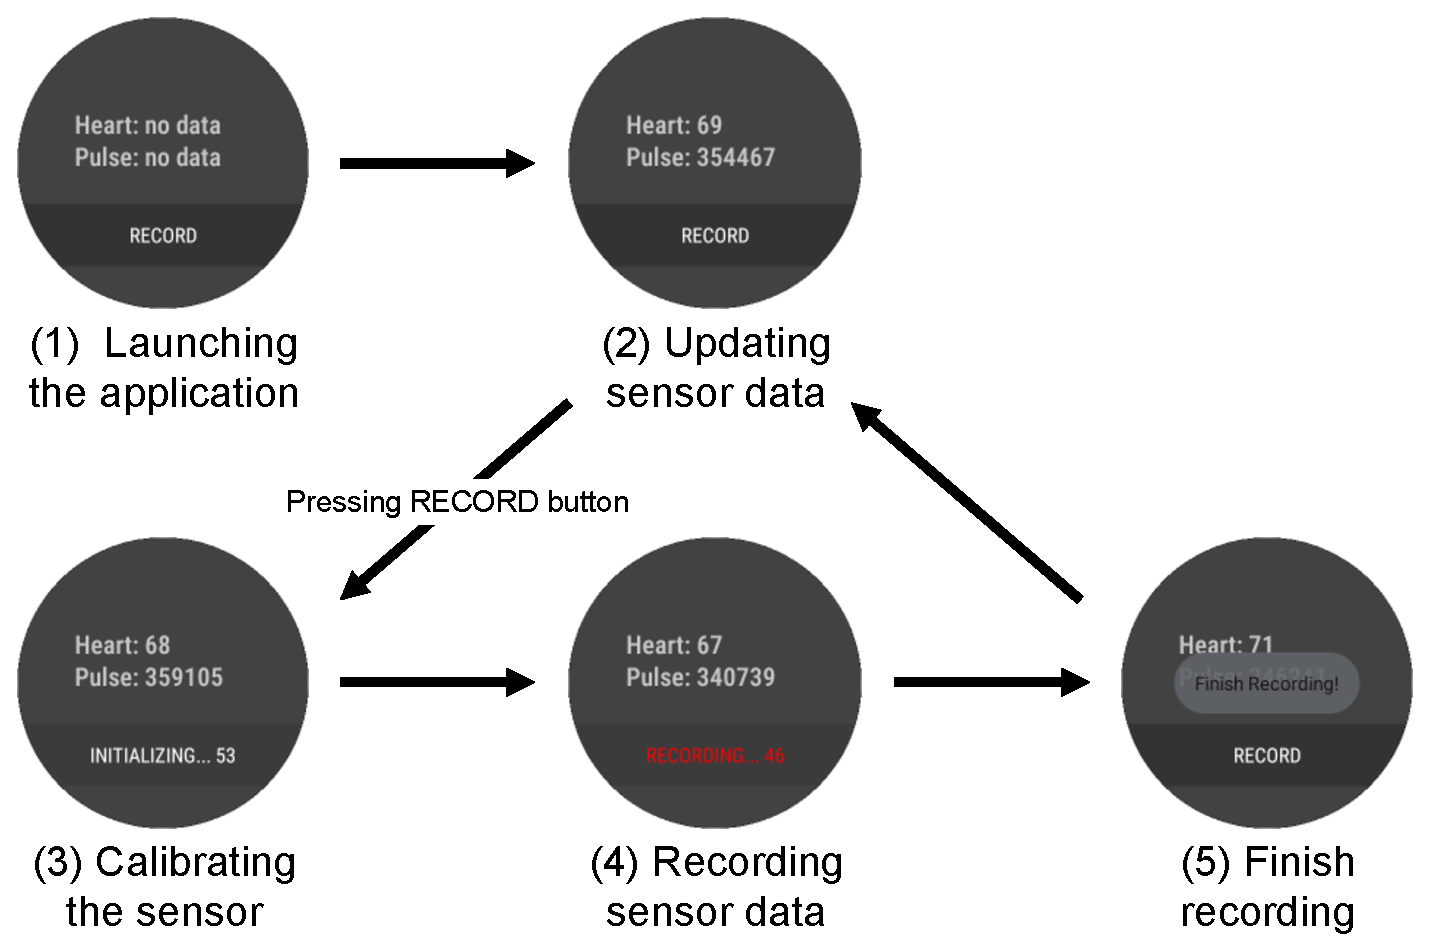
\includegraphics[width=1\linewidth]{figures/app.eps}
  \caption{Details of the implemented application.}
  \label{fig:app}
\end{figure}

\begin{figure}[!t]
  \centering
  \includegraphics[width=1\linewidth]{figures/calculate_heart_rate.eps}
  \caption{Calculation of heart rate for evaluation experiments with the smartwatches.}
  \label{fig:calculating_heart_rate}
\end{figure}

% 4.3.2
\subsubsection{watchOS}
\label{subsec:applewatch}
Apple Watch Series 3 and Series 5 were used in the experiment. Apple Watch comes standard with the Heart Rate app that measures heart rate\footnote{\url{https://support.apple.com/en-us/HT204666}}. The collected heart rate data can be output as numerical data in XML format using the iPhone ``Health'' application paired with Apple Watch\footnote{\url{https://support.apple.com/guide/iphone/share-health-and-fitness-data-iph27f6325b2/ios}}.\par

Data acquisition is started by placing the smartwatch on the display, entering the target heart rate into the standard input of the display drawing program, and launching the Heart Rate app. After a while, the Apple Watch display automatically turns off, and the heart rate acquisition is completed. The data acquisition time was not configurable, but the maximum time was approximately 160 seconds.\par

The sampling rate are not disclosed, and the number of data acquired in a single data acquisition process varies. In the evaluation experiment, as shown in the middle of \figref{calculating_heart_rate}, the first 30 seconds of data was excluded as calibration time, and the time average of the data for the following 60 seconds was calculated as the result of one heart rate. However, if there were no data acquired after the calibration time, the last data acquired was used as the resulting heart rate.

% 4.3.3
\subsubsection{Original OS}
\label{subsec:original}
The SMART R F-18 used in the experiment is equipped with a proprietary operating system developed by the manufacturer. Heart rate data collected by this smartwatch can be viewed on the ``WearHealth'' application developed for Android and iPhone\footnote{\url{https://play.google.com/store/apps/details?id=com.zjw.wearhealth}}\footnote{\url{https://apps.apple.com/us/app/wearhealth/id1265052549}}.\par

Data acquisition is started by placing the smartwatch on the display, entering the target heart rate into the standard input of the display drawing program, and operating the ``WearHealth'' application on the smartphone. After 30 seconds, the data acquisition was finished, and the resulting one heart rate was displayed on the application.\par

The sampling rate and the algorithm to determine the resulting heart rate are not disclosed. In the evaluation experiment, the one heart rate of the result displayed on the application, as shown in the bottom of \figref{calculating_heart_rate}, was recorded manually.


% 4.4
\subsection{Results and Discussion}
To obtain the correct heart rate, an acrylic plate of some thickness was placed between the display and a smartwatch in some display-smartwatch combinations. The display-smartwatch combinations and the thickness of the placed acrylic plate are shown in \tabref{acrylic_plate}. A blank cell indicates that the acrylic plate was not placed.\par

The smartwatches were placed on the display and the target heart rate was input to the display drawing program. The error of the measured heart rate was calculated by subtracting the measurement from the target, and that was taken as the result. The target heart rate was tested at intervals of 5 from 60 to 100 beats per minute (bpm), which is a resting heart rate range for adults\footnote{\url{https://www.heart.org/en/healthy-living/fitness/fitness-basics/target-heart-rates}}. The results of the evaluation experiment are shown in \tabref{result}, where the results are the average of three sets. Zero means that the heart rate was the same as the target heart rate, and minus means that the heart rate was smaller. $NaN$ indicates that the heart rate measurement has failed.\par

In addition, we conducted evaluation experiments using Display D with target heart rates set at 40--55 (heart rate during sleep) and 105--200 (heart rate during exercise). The results are shown in \tabref{result_expansion}.

\begin{table*}[!t]
  \small
  \centering
  \caption{The thickness of the placed acrylic plate.}
  \begin{tabular}{cccc|cccc|cccc|cccc|cccc}
  \toprule
    \multicolumn{4}{c|}{TicWatch Pro}&\multicolumn{4}{c|}{PUMA}&\multicolumn{4}{c|}{Series 3}&\multicolumn{4}{c|}{Series 5}&\multicolumn{4}{c}{SMART R} \\
    A & B & C & D & A & B & C & D & A & B & C & D & A & B & C & D & A & B & C & D \\
    \midrule
    -- & 2-mm & -- & 5-mm & -- & -- & -- & 2-mm & -- & -- & -- & -- & -- & 2-mm & -- & -- & 2-mm & -- & -- & -- \\
    \bottomrule
  \end{tabular}
  \label{tab:acrylic_plate}
\end{table*}

\begin{table*}[!t]
  \small
  \centering
  \caption{Error of resting heart rate obtained by TicWatch Pro, PUMA Smartwatch, Apple Watch Series 3, Apple Watch Series 5, and SMART R. (Display A: Lenovo Legion 7, B: 3.5-inch ELECROW, C: 3.5-inch OSOYOO, D: flexible display)}
  \begin{tabular}{c|cccc|cccc}
  \toprule
    &\multicolumn{4}{c|}{TicWatch Pro}&\multicolumn{4}{c}{PUMA} \\
    $H_{target}$ & A & B & C & D & A & B & C & D \\
    \midrule
    $60$ & $-1.7$ & $-1.4$ & $-1.4$ & $-2.0$ & $-1.7$ & $-1.4$ & $-1.4$ & $-0.8$ \\
    $65$ & $-1.8$ & $-1.4$ & $-1.3$ & $-2.5$ & $-1.8$ & $-1.4$ & $-1.3$ & $-1.8$ \\
    $70$ & $-1.8$ & $-2.1$ & $-1.2$ & $-0.4$ & $-1.8$ & $-2.1$ & $-1.2$ & $-0.9$ \\
    $75$ & $-2.2$ & $-1.6$ & $-1.5$ & $-0.1$ & $-2.2$ & $-1.6$ & $-1.5$ & $-1.2$ \\
    $80$ & $-2.0$ & $-1.5$ & $-1.1$ & $0.6$ & $-2.0$ & $-1.5$ & $-1.1$ & $0.0$ \\
    $85$ & $-1.8$ & $-1.5$ & $-1.6$ & $0.5$ & $-1.8$ & $-1.5$ & $-1.6$ & $0.3$ \\
    $90$ & $-2.0$ & $-1.7$ & $-1.0$ & $-0.4$ & $-2.0$ & $-1.7$ & $-1.0$ & $-0.5$ \\
    $95$ & $-2.0$ & $-1.2$ & $-1.1$ & $0.0$ & $-2.0$ & $-1.2$ & $-1.1$ & $-1.2$ \\
    $100$ & $-1.9$ & $-1.5$ & $-1.4$ & $-1.0$ & $-1.9$ & $-1.5$ & $-1.4$ & $-1.2$ \\
    \midrule
    Average & $-1.9$ & $-1.5$ & $-1.3$ & $-0.6$ & $-1.9$ & $-1.5$ & $-1.3$ & $-0.8$ \\
    \bottomrule
  \end{tabular}
  \begin{tabular}{c|cccc|cccc|cccc}
  \toprule
    &\multicolumn{4}{c|}{Series 3}&\multicolumn{4}{c|}{Series 5}&\multicolumn{4}{c}{SMART R} \\
    $H_{target}$ & A & B & C & D & A & B & C & D & A & B & C & D \\
    \midrule
    $60$ & $0.4$ & $1.0$ & $-0.2$ & $NaN$ & $58.2$ & $0.1$ & $-0.1$ & $0.0$ & $-1.7$ & $-1.0$ & $-1.7$ & $-0.7$ \\
    $65$ & $0.6$ & $0.1$ & $-0.1$ & $NaN$ & $16.1$ & $-0.4$ & $0.1$ & $0.0$ & $-1.7$ & $-1.0$ & $-0.7$ & $-0.7$ \\
    $70$ & $0.1$ & $2.0$ & $0.0$ & $NaN$ & $1.6$ & $2.4$ & $0.1$ & $0.0$ & $-1.0$ & $-1.3$ & $-1.3$ & $-0.7$ \\
    $75$ & $0.0$ & $2.8$ & $-0.6$ & $NaN$ & $0.8$ & $0.1$ & $-0.2$ & $-0.1$ & $-2.0$ & $-2.3$ & $-2.0$ & $-0.7$ \\
    $80$ & $-0.5$ & $1.0$ & $-0.5$ & $NaN$ & $1.2$ & $0.9$ & $-0.4$ & $-0.5$ & $-2.0$ & $-2.0$ & $-1.0$ & $-1.0$ \\
    $85$ & $-5.4$ & $-0.7$ & $-0.6$ & $NaN$ & $-0.6$ & $-1.0$ & $-0.9$ & $0.0$ & $-2.0$ & $-2.0$ & $-1.7$ & $-0.7$ \\
    $90$ & $-0.6$ & $-1.3$ & $-0.6$ & $NaN$ & $4.3$ & $-1.0$ & $-0.9$ & $0.0$ & $-3.3$ & $-2.3$ & $-1.7$ & $-1.0$ \\
    $95$ & $-1.5$ & $-0.5$ & $-1.0$ & $NaN$ & $-0.1$ & $-0.3$ & $-1.1$ & $0.0$ & $-2.7$ & $-2.0$ & $-2.0$ & $-0.3$ \\
    $100$ & $-0.7$ & $-1.1$ & $-0.7$ & $NaN$ & $-0.2$ & $-7.3$ & $-0.8$ & $-32.7$ & $-2.7$ & $-2.3$ & $-2.7$ & $-1.0$ \\
    \midrule
    Average & $-0.8$ & $0.4$ & $-0.5$ & $NaN$ & $9.0$ & $-0.7$ & $-0.5$ & $-3.7$ & $-2.1$ & $-1.8$ & $-1.6$ & $-0.7$ \\
    \bottomrule
  \end{tabular}
  \label{tab:result}
\end{table*}

\begin{table*}[!t]
  \small
  \centering
  \caption{Error of characteristic heart rate obtained by TicWatch Pro, PUMA Smartwatch, Apple Watch Series 3, Apple Watch Series 5, and SMART R. (Display D: flexible display)}
  \begin{tabular}{c|c|c|c|c|c}
  \toprule
    & TicWatch Pro & PUMA & Series 3 & Series 5 & SMART R \\
    $H_{target}$ & D & D & D & D & D \\
    \midrule
    $40$ & $0.0$ & $0.0$ & $NaN$ & $3.1$ & $23.7$ \\
    $45$ & $-1.2$ & $-1.0$ & $NaN$ & $0.1$ & $31.7$ \\
    $50$ & $-1.7$ & $-0.8$ & $NaN$ & $0.0$ & $0.3$ \\
    $55$ & $-0.7$ & $-0.7$ & $NaN$ & $0.0$ & $0.0$ \\
    \vdots & \vdots & \vdots & \vdots & \vdots & \vdots \\
    $105$ & $-0.2$ & $0.0$ & $NaN$ & $-34.3$ & $0.0$ \\
    $110$ & $-0.2$ & $0.0$ & $NaN$ & $-0.2$ & $-0.3$ \\
    $115$ & $-0.2$ & $0.3$ & $NaN$ & $-39.3$ & $-0.3$ \\
    $120$ & $-0.3$ & $-0.7$ & $NaN$ & $-41.5$ & $-0.7$ \\
    $125$ & $-0.8$ & $0.0$ & $NaN$ & $-0.7$ & $-0.3$ \\
    $130$ & $0.9$ & $0.3$ & $NaN$ & $-41.9$ & $0.0$ \\
    $135$ & $0.0$ & $-0.8$ & $NaN$ & $-41.7$ & $-0.3$ \\
    $140$ & $0.2$ & $-0.3$ & $NaN$ & $-70.7$ & $0.0$ \\
    $145$ & $0.7$ & $-0.2$ & $NaN$ & $-40.2$ & $0.3$ \\
    $150$ & $-0.1$ & $-0.3$ & $NaN$ & $-0.6$ & $-0.3$ \\
    $155$ & $0.5$ & $0.0$ & $NaN$ & $0.1$ & $0.0$ \\
    $160$ & $0.6$ & $0.0$ & $NaN$ & $0.0$ & $-0.3$ \\
    $165$ & $1.7$ & $1.3$ & $NaN$ & $0.0$ & $0.7$ \\
    $170$ & $0.0$ & $0.7$ & $NaN$ & $-94.4$ & $0.0$ \\
    $175$ & $0.3$ & $0.0$ & $NaN$ & $-50.6$ & $-0.7$ \\
    $180$ & $0.3$ & $0.6$ & $NaN$ & $-63.0$ & $0.0$ \\
    $185$ & $1.0$ & $-0.4$ & $NaN$ & $-0.3$ & $0.3$ \\
    $190$ & $1.4$ & $-0.2$ & $NaN$ & $-86.8$ & $0.3$ \\
    $195$ & $0.3$ & $1.7$ & $NaN$ & $-83.4$ & $0.3$ \\
    $200$ & $0.6$ & $0.0$ & $NaN$ & $-103.0$ & $0.0$ \\
    \bottomrule
  \end{tabular}
  \label{tab:result_expansion}
\end{table*}

% 4.4.1
\subsubsection{WearOS Smartwatch}
The results showed that the heart rate could be input to the smartwatch within an error of less than $3$ bpm. In both wearOS smartwatch results, the average error was smaller for Displays A, B, C, and D, in that order. This suggests that differences in performance, such as display brightness and refresh rate, may affect the generated heart rate.\par

Even when the characteristic heart rate was set as the target heart rate, the heart rate could be input to the smartwatch with a small error.

% 4.4.2
\subsubsection{WatchOS Smartwatch}
The results showed that using Display C enabled the heart rate to be input to the Apple Watch within an error of $-1.1$ to $0.1$ bpm. On the other hand, when using Display A or B, it was not possible to obtain the correct heart rate under some conditions. The correct heart rate was not obtained even once, when the target heart rate was set to 60 with the combination of Apple Watch Series 5 and Display A.\par

For the characteristic target heart rates, correct values were obtained for some target heart rates when using Apple Watch Series 5. When the target heart rate was set above 100, the obtained heart rate was very small compared to the target heart rate. It is possible that the large target heart rate was recognized by the Apple Watch algorithm as an incorrect heart rate and was calibrated to the resting heart rate.\par

The combination of Apple Watch Series 3 and Display D failed to measure the heart rate regardless of the target heart rate. Since the PPG sensor uses a photoreflector, they are easily affected by light, and depending on the condition of the position where the device is placed, the pulse data cannot be acquired correctly. Whether or not the generated pulse wave can be recognized by the smartwatch is thought to depend on the shape of the PPG sensor part of the device. The acrylic plate we prepared in this paper could not support Apple Watch Series 3, but there is a possibility that the pulse data can be input by placing a material of other materials and thickness.

% 4.4.3
\subsubsection{OriginalOS Smartwatch}
The results showed that the heart rate could be input to the smartwatch within an error of almost less than $3$ bpm. Especially for Display D, the heart rate could be input to the smartwatch within an error of less than $1$ bpm.\par

When the target heart rate was a characteristic heart rate, the heart rate could be input into the smartwatch with a very small error in many cases, but for target heart rates below 50, the heart rate could not be input correctly. This is thought to be due to the performance limitation of the PPG sensor in the smartwatch.



% 5
\section{Limitations}
\label{sec:limitation}
From the results in Section \ref{sec:evaluation}, the heart rate could be input into the smartwatch with small errors. This section discusses the limitations of the proposed method in terms of other pulse wave related indices and pulse wave waveform.\par

In order to compare, the real raw PPG data of the author's left index finger and the raw PPG data generated by Display D were acquired. The environment during raw pulse data acquisition is shown in \figref{raw_data_acquisition}. Numerical pulse data was collected at a sampling rate of 106 Hz for 60 seconds using Arduino Uno R3 and a PPG sensor manufactured by pulsesensor.com. The Arduino used here is a different one from the one used to control the display.

\begin{figure}[!t]
  \centering
  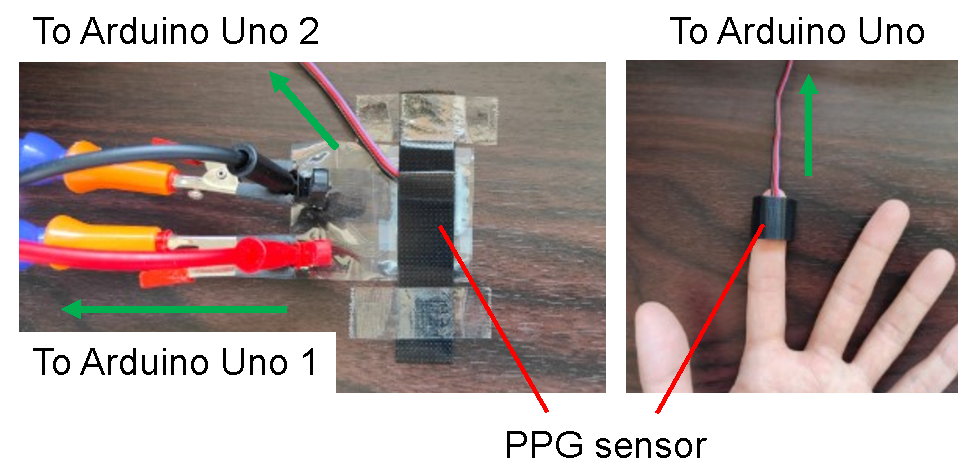
\includegraphics[width=1\linewidth]{figures/raw_data_acquisition.eps}
  \caption{The environment during raw pulse data acquisition.}
  \label{fig:raw_data_acquisition}
\end{figure}


% 5.1
\subsection{Pulse wave status indicators}
The raw PPG data obtained was analyzed using Kubios HRV Premium\footnote{\url{https://www.kubios.com/hrv-premium}}, a full featured Heart rate variability (HRV) analysis software for scientific research and professional use. \tabref{report_real} shows the results of analysis of the real PPG data, and \tabref{report_generated} shows the results of analysis of the generated PPG data. RR Time Series data are plotted in \figref{rr_wave}. The target heart rate at the time of pulse wave generation was set to 67 bpm, which is the same as the mean heart rate of the real pulse wave obtained from the finger. From the results, it can be seen that the generated pulse wave is 67 for both Min HR and Max HR, and the target heart rate can be input to the PPG sensor in a stable manner as in the evaluation experiment in section \ref{sec:evaluation}. RR interval was close and normal between the real and generated pulse waves, indicating that the generated pulse wave could be recognized as a correctly pulse wave waveform. SDNN of the generated pulse wave showed a very small value. SDNN is the standard deviation of RR interval, and since the mechanically generated pulse wave was a stable waveform, no variation in RR interval occurred and SDNN may have been small. The fact that there is no variation in RR intervals can be seen in \figref{rr_wave}. HF, also known as respiratory sinus arrhythmia (RSA), is the variation of RR interval with respiration. When HF is high, it indicates that the parasympathetic nervous system is dominant and respiratory cycle is regular. From Power (\%) and LF/HF ratio of the generated pulse wave, it can be seen that HF is very large and the mechanically generated pulse wave is a stable waveform without any turbulence.

\begin{table*}[!t]
  \small
  \centering
  \caption{Status evaluation index report of the real PPG data.}
  \begin{tabular}{lrr}
  \multicolumn{3}{c}{Time-Domain Results} \\
  \toprule
    Variable & Units & Value \\
    \midrule
    Mean RR & (ms) & $891$ \\
    Mean HR & (bpm) & $67$ \\
    Min HR & (bpm) & $65$ \\
    Max HR & (bpm) & $70$ \\
    SDNN & (ms) & $20.8$ \\
    RMSSD & (ms) & $22.1$ \\
    NN50 & (beats) & $1$ \\
    pNN50 & (\%) & $1.69$ \\
    RR triangular index & & $5.45$ \\
    TINN & (ms) & $89.0$ \\
    Stress Index (SI) & & $17.8$ \\
    DC & (ms) & $17.0$ \\
    DCmod & (ms) & $24.5$ \\
    \bottomrule
  \end{tabular}
  \begin{tabular}{lrrrr}
  \multicolumn{5}{c}{Frequency-Domain Results (FFT spectrum)} \\
  \toprule
    Variable & Units & VLF & LF & HF \\
    \midrule
    Frequency band & (Hz) & $0.00\text{--}0.04$ & $0.04\text{--}0.15$ & $0.15\text{--}0.40$ \\
    Peak frequency & (Hz) & $0.040$ & $0.050$ & $0.213$ \\
    Power & (ms${}^\text{2}$) & $54$ & $320$ & $192$ \\
    Power & (log) & $3.981$ & $5.767$ & $5.256$ \\
    Power & (\%) & $9.49$ & $56.58$ & $33.92$ \\
    Power & (n.u.) & & $62.51$ & $37.48$ \\
    \text{-}\text{-}\text{-}\text{-}\text{-}\text{-}\text{-}\text{-}\text{-}\text{-}\text{-}\text{-}\text{-} & & & & \\
    Total power & (ms${}^\text{2}$) & $565$ & & \\
    Total power & (log) & $6.337$ & & \\
    LF/HF ratio & & $1.668$ & & \\
    RESP & (Hz) & $-$ & & \\
    \bottomrule
  \end{tabular}
  \label{tab:report_real}
\end{table*}

\begin{table*}[!t]
  \small
  \centering
  \caption{Status evaluation index report of the generated PPG data.}
  \begin{tabular}{lrr}
  \multicolumn{3}{c}{Time-Domain Results} \\
  \toprule
    Variable & Units & Value \\
    \midrule
    Mean RR & (ms) & $895$ \\
    Mean HR & (bpm) & $67$ \\
    Min HR & (bpm) & $67$ \\
    Max HR & (bpm) & $67$ \\
    SDNN & (ms) & $2.4$ \\
    RMSSD & (ms) & $4.1$ \\
    NN50 & (beats) & $0$ \\
    pNN50 & (\%) & $0.00$ \\
    RR triangular index & & $1.67$ \\
    TINN & (ms) & $9.0$ \\
    Stress Index (SI) & & $67.0$ \\
    DC & (ms) & $1.1$ \\
    DCmod & (ms) & $4.1$ \\
    \bottomrule
  \end{tabular}
  \begin{tabular}{lrrrr}
  \multicolumn{5}{c}{Frequency-Domain Results (FFT spectrum)} \\
  \toprule
    Variable & Units & VLF & LF & HF \\
    \midrule
    Frequency band & (Hz) & $0.00\text{--}0.04$ & $0.04\text{--}0.15$ & $0.15\text{--}0.40$ \\
    Peak frequency & (Hz) & $0.040$ & $0.127$ & $0.253$ \\
    Power & (ms${}^\text{2}$) & $0$ & $0$ & $2$ \\
    Power & (log) & $0.000$ & $0.000$ & $0.874$ \\
    Power & (\%) & $0.15$ & $9.49$ & $90.20$ \\
    Power & (n.u.) & & $9.50$ & $90.33$ \\
    \text{-}\text{-}\text{-}\text{-}\text{-}\text{-}\text{-}\text{-}\text{-}\text{-}\text{-}\text{-}\text{-} & & & & \\
    Total power & (ms${}^\text{2}$) & $3$ & & \\
    Total power & (log) & $0.977$ & & \\
    LF/HF ratio & & $0.105$ & & \\
    RESP & (Hz) & $-$ & & \\
    \bottomrule
  \end{tabular}
  \label{tab:report_generated}
\end{table*}

\begin{figure*}[!t]
  \centering
  \includegraphics[width=0.8\linewidth]{figures/rr_wave.eps}
  \caption{RR Time Series data.}
  \label{fig:rr_wave}
\end{figure*}


% 5.2
\subsection{Pulse wave waveform}
The first 10 seconds of the obtained raw PPG data are plotted in \figref{raw_wave}. The real pulse wave varies in amplitude and is not stable, but the generated pulse wave is a stable waveform. However, the generated pulse waveform does not resemble the real pulse waveform, and the similarity between the waveforms is low. Even if the waveform is an irregular, it is recognized as a pulse wave by the smartwatch and analysis software, and indicators such as heart rate are calculated. Therefore, since the calculation of the pulse wave state indicators depends on the algorithm of each product, it is necessary to check the raw data waveform in order to verify that it is genuine PPG data.

\begin{figure*}[!t]
  \centering
  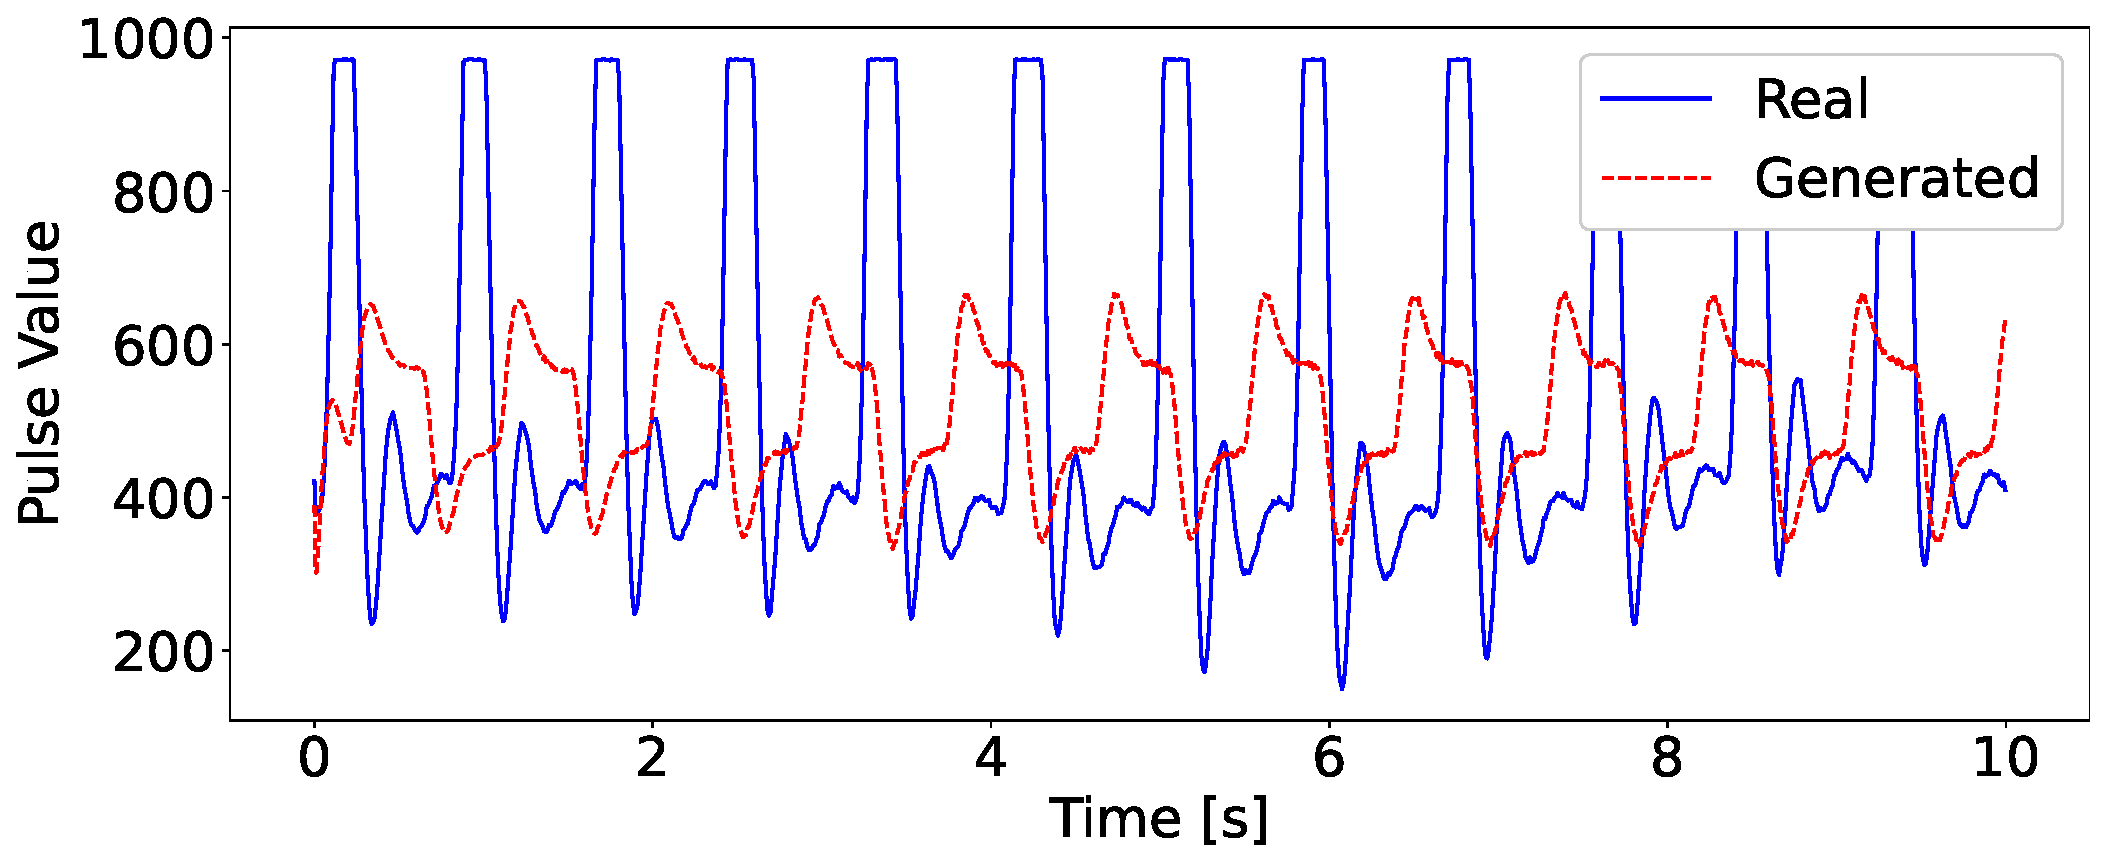
\includegraphics[width=0.8\linewidth]{figures/raw_wave.eps}
  \caption{Raw PPG data.}
  \label{fig:raw_wave}
\end{figure*}



% 6
\section{Conclusion}
\label{sec:conclusion}
In this paper, we proposed a method that enables a PPG sensor to measure arbitrary pulse wave using display. We implemented display drawing programs and conducted evaluation experiments using five kinds of smartwatches and four kinds of displays to determine the effectiveness of the proposed method. The results showed that the error between the target heart rate and the heart rate acquired by the smartwatch was within $3$ beats per minute in many cases when the target heart rate was set to 60--100. When the target heart rate was set to 40--55 and 105--200, the heart rate could be input to the smartwatch with a small error under some conditions. We compared the pulse wave status evaluation indices calculated from the real pulse wave obtained from the body and the generated pulse wave, and clarified that the pulse wave could be generated by the proposed method. By comparing the waveforms, the danger of calculating only the indices without checking the waveforms was clarified.\par

In future work, we will improve the reproducibility of PPG data for use in a real environment and implement a mechanism that enables the wearable device worn on the display to measure the same PPG data by inputting PPG data obtained from a live body part. To achieve this, the system needs to automatically determine the colors to be drawn on the display while calibrating for the environment, so we will build a generative model that can output the color to be drawn by inputting PPG data.



% \section{Acknowledgments}

% Identification of funding sources and other support, and thanks to
% individuals and groups that assisted in the research and the
% preparation of the work should be included in an acknowledgment
% section, which is placed just before the reference section in your
% document.

% This section has a special environment:
% \begin{verbatim}
%   \begin{acks}
%   ...
%   \end{acks}
% \end{verbatim}
% so that the information contained therein can be more easily collected
% during the article metadata extraction phase, and to ensure
% consistency in the spelling of the section heading.

% Authors should not prepare this section as a numbered or unnumbered {\verb|\section|}; please use the ``{\verb|acks|}'' environment.

% \section{Appendices}

% If your work needs an appendix, add it before the
% ``\verb|\end{document}|'' command at the conclusion of your source
% document.

% Start the appendix with the ``\verb|appendix|'' command:
% \begin{verbatim}
%   \appendix
% \end{verbatim}
% and note that in the appendix, sections are lettered, not
% numbered. This document has two appendices, demonstrating the section
% and subsection identification method.

% \section{SIGCHI Extended Abstracts}

% The ``\verb|sigchi-a|'' template style (available only in \LaTeX\ and
% not in Word) produces a landscape-orientation formatted article, with
% a wide left margin. Three environments are available for use with the
% ``\verb|sigchi-a|'' template style, and produce formatted output in
% the margin:
% \begin{itemize}
% \item {\verb|sidebar|}:  Place formatted text in the margin.
% \item {\verb|marginfigure|}: Place a figure in the margin.
% \item {\verb|margintable|}: Place a table in the margin.
% \end{itemize}

%%
%% The acknowledgments section is defined using the "acks" environment
%% (and NOT an unnumbered section). This ensures the proper
%% identification of the section in the article metadata, and the
%% consistent spelling of the heading.
% \begin{acks}
% To Robert, for the bagels and explaining CMYK and color spaces.
% \end{acks}

%%
%% The next two lines define the bibliography style to be used, and
%% the bibliography file.
\bibliographystyle{ACM-Reference-Format}
\bibliography{references}

%%
%% If your work has an appendix, this is the place to put it.
% \appendix

% \section{Research Methods}

% \subsection{Part One}

% Lorem ipsum dolor sit amet, consectetur adipiscing elit. Morbi
% malesuada, quam in pulvinar varius, metus nunc fermentum urna, id
% sollicitudin purus odio sit amet enim. Aliquam ullamcorper eu ipsum
% vel mollis. Curabitur quis dictum nisl. Phasellus vel semper risus, et
% lacinia dolor. Integer ultricies commodo sem nec semper.

% \subsection{Part Two}

% Etiam commodo feugiat nisl pulvinar pellentesque. Etiam auctor sodales
% ligula, non varius nibh pulvinar semper. Suspendisse nec lectus non
% ipsum convallis congue hendrerit vitae sapien. Donec at laoreet
% eros. Vivamus non purus placerat, scelerisque diam eu, cursus
% ante. Etiam aliquam tortor auctor efficitur mattis.

% \section{Online Resources}

% Nam id fermentum dui. Suspendisse sagittis tortor a nulla mollis, in
% pulvinar ex pretium. Sed interdum orci quis metus euismod, et sagittis
% enim maximus. Vestibulum gravida massa ut felis suscipit
% congue. Quisque mattis elit a risus ultrices commodo venenatis eget
% dui. Etiam sagittis eleifend elementum.

% Nam interdum magna at lectus dignissim, ac dignissim lorem
% rhoncus. Maecenas eu arcu ac neque placerat aliquam. Nunc pulvinar
% massa et mattis lacinia.

\end{document}
\endinput
%%
%% End of file `sample-authordraft.tex'.
